\chapter{Applications}
\label{chap:clients}

In Chapter \ref{chap:purpose} I discussed several potential
applications for Custos. In Chapter \ref{chap:platform} I discussed
the Custos architecture and server API. In this chapter, I'll look
more closely at several example applications that interface with the
Custos server and leverage Custos to enhance their functionality. As
with the implementations provided in Chapter \ref{chap:platform},
these applications are designed merely to serve as examples of how one
might leverage Custos. They are by no means intended to represent a
complete list of all possible Custos applications. Nor are they
designed as fully production ready systems. They are proofs of concept
that demonstrate how to use Custos and the features using Custos
brings.

\section{\texttt{EncFS}: A Custos-backed Encrypted File System}

As discussed, encrypted file systems are a core Custos use case. As
such, I have written a layered, encrypted pass-through file system:
\texttt{EncFS}. This file system leverages Custos for encrypted file
key storage, and leverage underlying file systems for encrypted file
storage. It enables use cases not normally available in other
encrypted file systems.

The file system is capable of supporting encrypted operation in a wide
range of scenarios. Since it is a pass-through file system, it can be
used atop Cloud storage systems like Dropbox~\cite{dropbox}, secure
storage of a users files in the cloud. Custos enables access to the
encrypted files from multiple devices or by multiple users, allowing a
user to use Dropbox as they normally would to sync files across
multiple devises or to share files with other, all while still
benefiting from encryption.

The system can also be used atop a users local file system, guarding
against data compromise in the event that the users computer is lost
or stolen. In addition, the file system has proven useful for use on
servers, where Custos's flexible authentication systems can allow for
daemon-based non-interactive access. This has allowed me to encrypt
server files like logs or mailboxes that normally must not be
encrypted in order to per-server non-interactive access by system
processes.

\subsection{Architecture}

\begin{figure}[!tb]
  \vspace{5ex}
  \begin{center}
    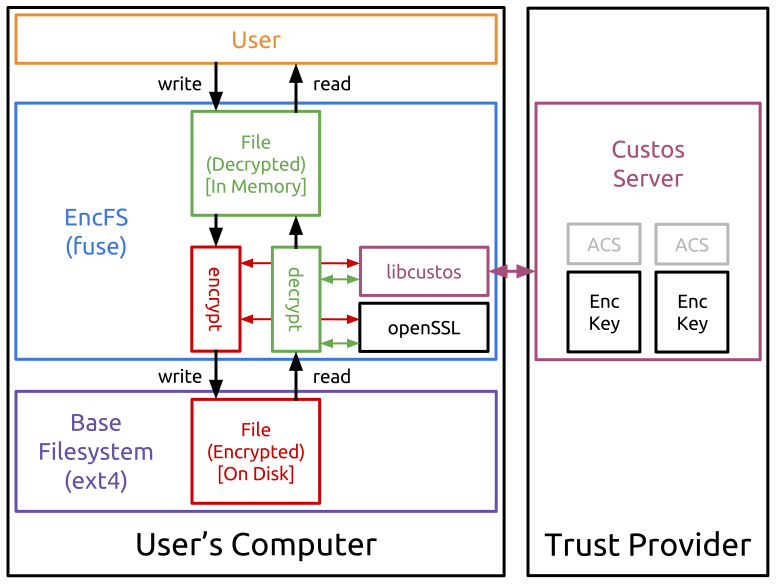
\includegraphics[width=.75\textwidth]
                    {./figs/pdf/App-FS-Fuse.pdf}
  \end{center}
  \caption{The \texttt{EncFS} File System Architecture}
  \label{fig:app-encfs}
\end{figure}

As Figure \ref{fig:app-encfs} shows, \texttt{EncFS} uses an
architecture similar to that described as the ``layered model'' in
Chapter \ref{chap:purpose}. It acts as a shim between user file system
operations (read, write, create, etc) and the actual realization of
these operations on the underlying file system, proving transparent
encryption in between. If the user attempts to read a file directly
from disk without first passing through the \texttt{EncFS} layer, they
will only received encrypted gibberish. But when the same file is
accessed through the \texttt{EncFS} layer, the user may interact with
the file as though it were not encrypted. As such, the user's files
are fully protected when the \texttt{EncFS} layer is not mounted or
not running, and easily accessible when this layer is mounted or is
running.

At this time \texttt{EncFS} only provides file encryption, not file
organization encryption. This is sufficient to demonstrate how to use
Custos to secure an encrypted file system, while avoiding the
complexity of also encrypting file system organization. When a user
wishes to start \texttt{EncFS}, they specify a mount point and a base
file system point. The base file system point become the root on the
\texttt{EncFS} backing file system. Any files accessed via the
\texttt{EncFS} mount point are actually stored/accessed at the
underlying base file system point. \texttt{EncFS} simply provides a
means for adding and removing encryption between the actual storage of
files on the underlying file system and the corresponding access to
files on the part of a user.

Because file systems do nor normally provide means for interactive
authentication, all necessary authentication parameters must be based
to \texttt{EncFS} at the time it is mounted/started. If a user tires
to access a file for which the combination of provided and implicit
authentication attributes are not sufficient, they are simply denied
access to the file. \texttt{EncFS} itself does to provide the ability
to manipulate Custos Access Control Specifications. Instead, this
manipulation is handled by a separate, dedicated utility program (see
below). As long as the user has the necessary permissions, all
encrypted file access via \texttt{EncFS} is fully transparent,
allowing easy integration with other applications via the started
Linux file interface~\cite{linux-vfs}.

\subsection{Implementation}

\texttt{EncFS} is implemented using the FUSE~\cite{fuse}. I chose a
FUSE-based implementation over a native Linux kernel-module
implementation for \texttt{EncFS} in order to allow easy usage of a
variety of user-space libraries (i.e. \texttt{libcustos}, OpenSSL,
etc). The basics of using FUSE to create an virtual overlay file
system like \texttt{EncFS} are described in my previous work:
~\cite{sayler-os-encfs}. FUSE provides a series of callbacks that are
triggered by various file system operations. Each callback is then
implemented by \texttt{EncFS} in C in order to provided the desired
encryption functionality.

All encryption in \texttt{EncFS} uses the AES symmetric encryption
cipher with 256-bit keys and the CBC encryption mode. Encryption
operations are handled by the OpenSSL~\cite{openssl} crypto
library\footnote{Following the old adage that one should never ``roll
  their own'' crypto. Leave it to the professionals! (Or at least to a
  widely used, well vetted code base.)}. Data written via the
\texttt{EncFS} mount point is encrypted before being committed to an
actual file on the underlying disk. Likewise, data read via the
\texttt{EncFS} mount point is decrypted before being passed back to
the user. This includes decrypting files when the user accesses
related meta-data like file size to ensure the user receives the size
of the unencrypted file content. Currently, \texttt{EncFS} encrypted
files in single blocks, meaning the entire file must be read to
decrypt any portion of it. This can have an adverse effect on access
to random offsets within a file. I plan to upgrade the system to
support breaking files into blocks in order to speed random access and
streaming operations in the near future.

\texttt{EncFS} interacts with Custos via the \texttt{libcustos}
library (see Chapter \ref{chap:platform}). This allows \texttt{EncFS}
to overlaid the complexities of the Custos API to a dedicated code
base. \texttt{libcustos} provides the necessary functions to allow
\texttt{EncFS} to read, update, and create Custos key:value
objects. When a user wishes to decrypt a file, \texttt{EncFS}
requested the associated encryption key form the Custos server using
the UUID stored with the file (either via extended attributes or in a
header block appended to the encrypted file contents, depending on
system support for extended attributes). If \texttt{EncFS} posses the
necessary authentication attributes (either supplied by the user at
mount time or derived contextually), Custos return the request key and
\texttt{EncFS} proceeds to decrypt the file. The opposite operation
occurs when a file is created or written, with \texttt{EncFS} rotating
the encryption key and uploading a new version to Custos for each
write operation.

\section{ACS Management UI}

In order to make Custos data easy to manage while developing various
Custos apps that lack built-in management capabilities, I've designed
a basic managed user interface that simplifies the process of
interacting with the Custos server and managing the Access Control
Specification associated with a given Custos key:value object.

\subsection{Architecture}

\begin{figure}[!tb]
  \vspace{5ex}
  \begin{center}
    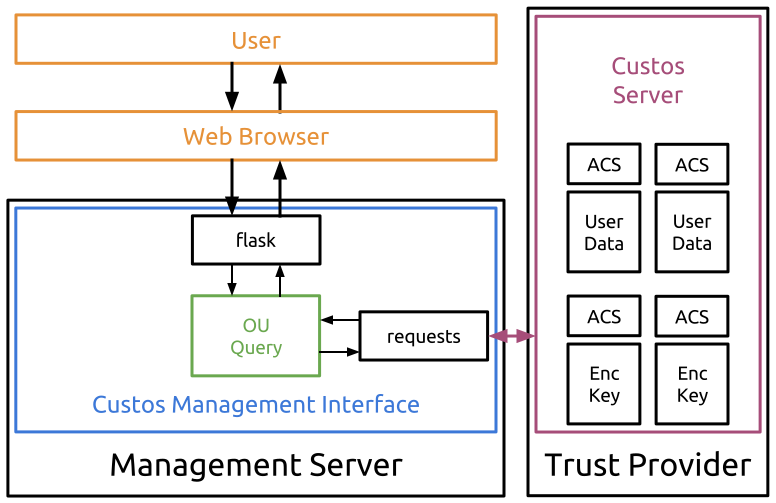
\includegraphics[width=.75\textwidth]
                    {./figs/pdf/App-Mgmt.pdf}
  \end{center}
  \caption{The ACS Management Architecture}
  \label{fig:app-mgmt}
\end{figure}

The management interface utilizes a web-based UI for managing Custos
access control specifications (Figure \ref{fig:app-mgmt}). The user
access the UI by ``logging in'' through the prevision of one or more
authentication attributes. The UI stores these attributes in the user
restyling session state, and leverages them to grant the user access
to verify Custos key:value ACSs. The user must have the appropriate
management permissions in order to make effective use of the
management UI.

Once ``logged in'', the user can input a UUID identifying a Custos
key:value object. They may then view the current ACS associated with
the object in JSON, and make any changes required before re-uploading
the object to Custos. It is possible to list multiple objects in order
to perform batch changes. The user is also capable of setting the
default ACS applied to newly created objects.

The management interface could also be coded as a command line utility
with fairly minimal changes. The interface would be similar, just via
command line interaction instead of a web UI. Neither system is ideal
for large scale, production Custos management, but both are adequate
for basic Custos management while testing or using the system with a
small number of users.

Custos's flexible authentication system also allows the administrator
to setup Custos to allow management access to any request from a
specific IP, making it simple to designate a management machine hat
can fully control Custos access without requiring more complex
attributes. This method has been sued effectively to provide
\texttt{local-host} to a Custos server to expedite management of
server data while developing against it.

\subsection{Implementation}

The web UI is implemented in Python 2.7 using the
Flask~\cite{python-flask} microframework (similar to the process
format used to implement the Custos server in Chapter
\ref{chap:platform}, but with actual UI elements instead of just a
JSON API). The application communicates with the Custos server via the
Python requests~\cite{python-requests} module. Python's numerous
modules handling JSON processing, deigning, etc making interfacing a
Python application directly whit the Custos server far easier than
implementing a C application. Thus, no specialized library
(i.e. \texttt{libcustos}) is necessary.

When a user request to view the ACS for a one or more objects, the
back-end builds the necessary Custos message and issues the request,
appending the user supplied authentication attribute. If the user has
the necessary permissions to view and edit an ACS, the ACS is
returned. The user can manipulate the existing ACS directly, and if
she desires, send it back to Custos, replacing the original ACS. This
system, while not the most polished, provides the user with the
ability to fully manipulate the ACS for any Custos stored object.

\section{``Banking'' Website}

\subsection{Architecture}

\begin{figure}[!tb]
  \vspace{5ex}
  \begin{center}
    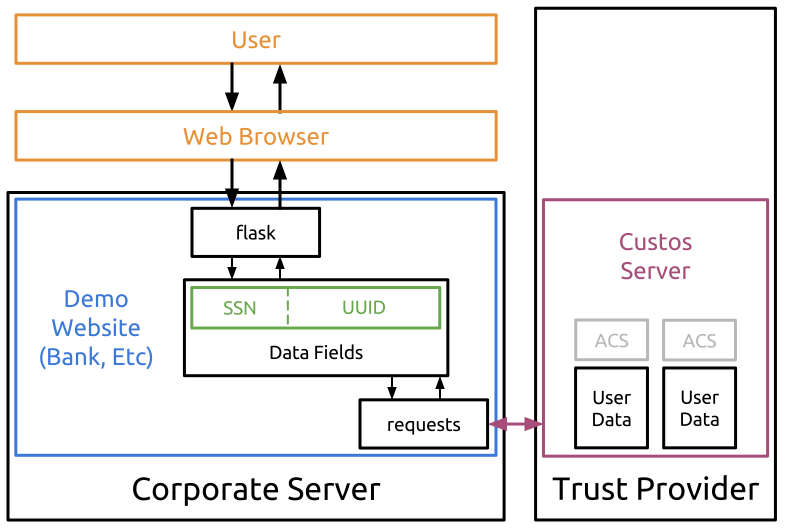
\includegraphics[width=.75\textwidth]
                    {./figs/pdf/App-SS.pdf}
  \end{center}
  \caption{The Demo ``Banking'' Website Architecture}
  \label{fig:app-bank}
\end{figure}

Public, Encrypted Personal Data Store

(Name, SSN, Etc)

\subsection{Implementation}

Static Encrypted Web Content

Assessor used Custos Client

%%  LocalWords:  EncFS libcustos OpenSSL ACSs ACS
